\chapter{Design and Implementation} \label{ch:framework}

Once the initial research was completed on the basics of blockchain and the current stage of the development of \gls{ssi} models, the objective of this thesis was developed. The 
first goal is to make the standalone framework for the decentralized user identity management, applying the \gls{ssi} models with the blockchain technology as the foundation. In 
this model, the identity management process consists of authentication and authorization procedures that do not rely on centralized systems or databases. The blockchain 
technology, smart contracts, and \gls{vc}s are used for this purpose. Therefore, it guarantees a high level of seclusion and security for the personal and 
sensitive information of the users.

Subsequently, the aim was to integrate this system into an ongoing project at Links Foundation named Data Cellar. Chapter \hyperref[ch:integration]{7} will delve into what Data Cellar is and discuss 
the integration of the framework into that project. 

In this chapter instead, the work will be analyzed in the design and implementation of the standalone framework for decentralized identity management. The work comprised 
several phases: analysis of existing projects in this domain, selection of the environment and libraries for developing the project, actual implementation of the project, 
and analysis of its limitations arising from the lack of robust support structures not yet commercially available, given the relatively short time since the development of 
blockchain-based \gls{ssi} systems.

\section{Framework Development Journey}

In this section, the design phase of the standalone framework is explored, tracing the journey from initial research to the final selection concerning the development 
environment, namely the blockchain and libraries for managing \gls{did}s. The choices made regarding the management of another fundamental element of the \gls{ssi} model, namely \gls{vc}s, 
will be discussed in section \hyperref[sec:6.3]{6.3}.

\subsection{Initial Research}

Firstly, we conducted an examination of the primary \gls{idms} blockchain products on the market. Several scientific papers and articles were examined to identify their technology
choices, means of operation, and functionalities they offer \cite{9315899}, \cite{9129332}, \cite{8776589}. The three primary solutions encountered were:

\begin{itemize}
  \item \textbf{ShoCard}: This \gls{ssi} technology underlines the decentralization providing every user with full control over their identities and data. \textit{ShoCard} uses the public 
  Bitcoin blockchain for digital identity and authentication, when users hold their identities on their devices using private keys.
  \item \textbf{The Sovrin Network}: Governed by \textit{Sovrin Foundation}, it is an open-source solutions framework that provides users with sovereign and decentralized digital 
  identities. It uses Sovrin ledger as a blockchain to support \textit{Hyperledger Indy} framework and other \textit{Hyperledger} libraries like \textit{Aries} and \textit{Ursa}.
  \item \textbf{The uPort System}: An open-source identity system management with \gls{ssi}. It uses Ethereum blockchain for identity representation and 
  \gls{ipfs} for data storing.
\end{itemize}

\renewcommand{\arraystretch}{1.4}
\begin{table}[h]
  \centering
  \begin{tabularx}{\textwidth}{|>{\centering\arraybackslash}m{3.3cm}|>{\centering\arraybackslash}m{3.2cm}|>{\centering\arraybackslash}m{3.2cm}|>{\centering\arraybackslash}m{3.2cm}|}
    \hline
    \thead{Project} & \thead{ShoCard} & \thead{Sovrin} & \thead{uPort} \\
    \hline
    Blockchain Implementation & Bitcoin & Hyperledger Indy & Ethereum \\
    \hline
    Blockchain Type & Permissioned & Public Permissioned & Permissionless  \\
    \hline
    Storage & Off-Chain & On/Off-Chain & Off-Chain  \\
    \hline
    Interoperability & Yes & Yes & Yes  \\
    \hline
    Selective Disclosure & No & Yes & Yes  \\
    \hline
    Auth & Yes & Yes & No  \\
    \hline
  \end{tabularx}
  \caption{A comparative analysis of blockchain based SSI system.}
\end{table}

In order to avoid the usage of the existing systems and to bring up a decentralized identity management system from scratch, the main work was done on the fundamentals. The 
first step was the creation of a unique user representation that in the case of a decentralized system is ensured by the \gls{did}s. Several libraries facilitating \gls{did} creation 
and management were explored \cite{10218198}, including:

\begin{itemize}
  \item \textbf{Ethr-did}: Utilizes Ethereum's accounts and smart contracts to implement the registry for \gls{did}s resolution. It stores \gls{ddo} on the Ethereum blockchain.
  \item \textbf{Did-algo}: A framework for the \textit{Algorand} blockchain, storing \gls{ddo}s on \gls{ipfs}. It offers a \gls{cli} software for managing operations and supports various 
  cryptographic keys.
  \item \textbf{Did-indy}: Part of the \textit{Hyperledger Indy} ecosystem, based on a permissioned blockchain with multiple logical ledgers. It enables role assignment to \gls{did}s and 
  provides mechanisms for \gls{vc} issuance and verification.
\end{itemize}

\subsection{Challenges and Failed Attempts}

Initially, there were works focusing on the analysis of the \textit{Did-indy}, which is also built on the \textit{Hyperledger Indy} blockchain. Nevertheless, the development was challenged 
by the outdated \textit{Indy} \gls{sdk} and the absence of the comprehensive guideline. 

These constraints thus provoked an exploration of other solutions, which resulted in a focus on \textit{algo-did}, which works on the \textit{Algorand} blockchain. It turns out that 
there were certain challenges that we encountered with \textit{algo-did}, such as documentation issues, technical problems that remain unresolved, and the lack of community 
support that we have noticed. These problems led to a re-evaluation of the relevance of this system for the framework.

\subsection{Final Choice}

After a thorough screening and exclusion process, the spotlight focused on \textit{ethr-did}, which is based on the Ethereum blockchain, one of the most widely used blockchains at 
present. The \textit{ethr-did} system was not only robust but also well-documented, and \textit{uPort} also made use of it, as discussed before, which made it the ideal option. 

In the beginning, the \textit{ethr-did} library's functionality was tested by running locally executed software, using \textit{Infura} to communicate with the Ethereum blockchain. 
Developers can easily get access to the blockchain networks through \textit{Infura} by creating an \gls{api} key, and this is done without requiring them to directly manage 
full nodes on their devices \cite{infura}.

However, anticipating the integration of the framework with the Data Cellar project, envisioned as a browser-accessible application for users, the framework was promptly developed 
in the form of a browser \gls{dapp} supported by the use of MetaMask. MetaMask serves not only as a digital wallet for users but also facilitates direct communication with the 
blockchain through the browser, eliminating the need for an \gls{api} key and thus \textit{Infura}.

\section{Framework Main Components}

In this section, the libraries, blockchain, and support tools utilized in the development of the standalone framework designed as a browser \gls{dapp} for 
identity management will be explored. This framework operates under the decentralized identity management model based on blockchain technology, focusing on the creation and 
management of \gls{did}s. The section excludes the management of \gls{vc}s, which will be addressed in the subsequent section.

\subsection{Ethr-did and Other Libraries}

The foundation for standalone framework development is \textit{ethr-did} library. Through \textit{ethr-did}, we try to use Ethereum addresses as a fully self-directed \gls{did} 
so as to help easy key development and management for these identifiers. \textit{ethr-did} standardizes the identity methods and provides a scalable mechanism for 
public keys and Ethereum addresses \cite{ethr-did}. Thus, the collection of on-chain and off-chain data becomes possible. 

This library relies on two additional libraries: 

\begin{itemize}
  \item \textbf{ethr-did-registry}: This library contains the Ethereum contract code allowing owners of \textit{ethr-did} identities to update attributes in their \gls{ddo}s. 
  It provides an \gls{api} enabling developers to interact with the contract functions using JavaScript, designed for resolving public keys for off-chain authentication \cite{ethr-did-registry}.
  \item \textbf{Ethr-did-resolver}: Intended for use with Ethereum addresses or secp256k1 public keys as fully self-managed \gls{did}s, wrapping them in a \gls{ddo}. It 
  supports the \gls{did}s spec from the W3C Credentials Community Group and relies on the \textit{did-resolver} library \cite{ethr-did-resolver}.
\end{itemize}

\textit{ethr-did} together with \textit{ethr-did-registry} and \textit{ethr-did-resolver} are all based on \textit{ethers}, which is a thin and well-known library for smart contract interactions and 
\gls{dapp}s development, most commonly used for digital wallets, like MetaMask.

The other hand, \textit{ethr-did} makes use of the \textit{did-jwt} library thereby introducing the signing and verification of \gls{jwt}s using various algorithms. However, specific 
functions from \textit{did-jwt} were not utilized in the framework created. 

In this case, only the \textit{ethr-did} constructor was used to generate \gls{did}s associated with users' Ethereum accounts and resolved them later using the \textit{ethr-did-resolver} library. 
Supplementary functions within \textit{ethr-did} were unnecessary for the purposes and thus remained unused.

\subsubsection{Ethr-did Constructor}

The majority of functions within the \textit{ethr-did} library can be executed either locally or interact directly with the Ethereum blockchain, depending on the chosen approach for 
constructing the \textit{ethr-did} object, whether or not the etherDidController class from the \textit{ethers} library. 

Now, let's analyze in detail the parameters required by the constructor \cite{ethr-did}: 

\begin{itemize}
  \item \textbf{identifier}: Represents the identifier used for \gls{did} creation, which can be either an Ethereum address, a public key, or an Ethereum address as a string. (Required)
  \item \textbf{chainNameOrId}: Represents the name or ID of the blockchain network. (Optional)
  \item \textbf{registry}: Represents the address of the \gls{did} registry contract. (Optional)
  \item \textbf{signer}: Represents the \gls{jwt} signer. (Optional)
  \item \textbf{alg}: Represents the signature algorithm, which can be either 'ES256K' or 'ES256K-R'. (Optional)
  \item \textbf{txSigner}: Represents the transaction signer. (Optional)
  \item \textbf{privateKey}: Represents the private key associated with the Ethereum address. (Optional)
  \item \textbf{rpcUrl}: Represents the RPC URL used to connect to the Ethereum network. (Optional)
  \item \textbf{provider}: Represents the Ethereum provider. (Optional)
  \item \textbf{web3}: Represents the web3 provider. (Optional)
\end{itemize}

The constructors logic checks, for the existence of an Ethereum provider or network details. If present, sets up the \textit{txSigner} using an object that can sign transactions or 
generates one, from a \textit{Wallet}. If a private key is defined and theres no existing \textit{txSigner} object a fresh \textit{Wallet} object is generated with the given key, which is then 
utilized as the \textit{txSigner} for signing transactions.

The \textit{EthrDidController} class is created to work with the ERC1056 contract, which's a standard used to represent identities, on the Ethereum platform. When the \textit{EthrDid} 
object constructor is called it triggers the constructor of \textit{EthrDidController} generating a \gls{did} with \textit{did:ethr} on the designated network, in a process. This means that only 
\gls{did}s generated through \textit{EthrDidController} and actions executed using its functions are able to communicate with the Ethereum network.

\subsection{Ethereum and Smart Contracts}

As previously mentioned, for the purpose of building the following framework of decentralized identity management, the Ethereum blockchain has been chosen. Ethereum is 
possibly one of the most widely used blockchains in the world today due to the fact that it has completely redefined the concept of blockchain itself through the functions 
of smart contracts and through the support for the development of \gls{dapp} \cite{ethereum}.

In particular, Ethereum's main test networks, namely \textit{Goerli} and \textit{Sepolia}, were used, given the possibility of obtaining the relevant tokens via faucets. A smart contract was 
set up on these blockchains to serve as a registry, for keeping track of which \gls{did}s linked to users Ethereum accounts had registered on the browser \gls{dapp}. In 
addition, the smart contract used by \textit{ethr-did} for managing \gls{did}s, which is useful during their resolution, already present on \textit{Goerli}, has also been 
deployed on \textit{Sepolia}.

Deployment of these contracts on \textit{Goerli} and \textit{Sepolia} will be facilitated by using \textit{Truffle}, a development framework for Ethereum that eases and hastens the creation of smart 
contracts and \gls{dapp}s. After correctly configuring \textit{Truffle} \cite{truffle-suite}, a brief script was created to deploy the contract, using the following commands: 

\begin{itemize}
  \item \textbf{"truffle compile"}: to compile the contract and obtain the \gls{abi}, which describes the methods it accepts, the parameters they accept, and the values returned.
  \item \textbf{"truffle migrate --network"}: to deploy the contract correctly on the given blockchain network, provided that the account used has enough tokens to cover 
  the fees. During deployment, the address of the block where the contract had been stored on the blockchain was retrieved.
\end{itemize}

\newpage

\lstinputlisting[language=JavaScript, caption={Deploying DataCellarRegistry contract.}]{Codes/deploy.js}

\subsubsection{The Smart Contract}

A smart contract is a self-executing contract wherein the conditions of the agreement are automatically captured in code. It executes the agreement conditions automatically 
and intermediaries are no longer a necessity. 

In the scope of the project, Solidity language is used to write a smart contract that will perform functions of user registration management in a decentralized way. It is 
realized by updating a mapping in which a boolean value is attached to each Ethereum account to show the user status whether he is registered or not. In using the Ethereum 
blockchain which is inherently decentralized and immutable, the Smart contract ensures the integrity and transparency of the system, while eliminating the need for a central
authority. Participants can register or unregister themselves safely and autonomously, with the contract recording these actions on the blockchain. 

Functions of the smart contract:

\begin{enumerate}
  \item \textbf{registerUser(address \_userAddress)}: It registers a user in the registry. This function can only be called by the user, and the user must not be already registered.
  \item \textbf{unregisterUser(address \_userAddress)}: Unregisters the user. This function can be called only by the user itself, and the user should have registered before that.
  \item \textbf{isUserRegistered(address \_userAddress)}: Checks if a user is registered in the registry. This function can be used by anyone, and it returns a boolean 
  value indicating whether the user is registered or not.
\end{enumerate}

The contracts three functions all require an Ethereum account as input. The final function is read only displaying whether a user is registered or not while the other two 
functions alter the contracts state. These state altering functions need the contract to update its status on the blockchain leading to transaction fees being paid to 
miners for overseeing and validating these modifications.

\lstinputlisting[language=Solidity, caption={Smart contract for DataCellarRegistry.}]{Codes/registry.sol}

\subsection{MetaMask}

One of the crucial factors that led to the construction of the framework as a browser \gls{dapp} is MetaMask. MetaMask is a user-friendly Ethereum blockchain software 
wallet designed for convenient transaction operations \cite{metamask}. In other words, MetaMask serves as an interface between the users and Ethereum \gls{dapp}s, providing access to Ethereum 
wallets via browser extensions or mobile applications. The advent of MetaMask has provided users with a convenient way to manage their cryptocurrencies, transact online, 
and engage \gls{dapp} across different browsers and mobile platforms. 

Specifically, the browser \gls{dapp} is able to monitor the presence of the MetaMask extension in the browser being used and the existence of an Ethereum 
account in the wallet, which most of the time means that the extension is connected to the application. Additionally, the \gls{dapp} can identify the primary account and the 
desired reference networks on MetaMask in real-time. As a matter of fact, MetaMask not only help in handling multiple accounts but also multiple network like \textit{Goerli} and 
\textit{Sepolia} which has been deployed the smart contract.

Finally, MetaMask provides the ability to securely store the private keys of \gls{dapp} accounts in a secure wallet, allowing users to sign and execute transactions that will 
enable them to register or deregister without the private keys ever leaving the extension in clear or encrypted form.

\lstinputlisting[language=JavaScript, caption={Function for updating wallet and accounts.}]{Codes/mm.js}

\section{Verifiable Credentials and Limitations} \label{sec:6.3}

As outlined in section \hyperref[sec:4.3]{4.3}, \gls{vc}s are crucial, in the \gls{ssi} model. So, once the blockchain and libraries for \gls{did} support were determined, the focus of the 
research turned to finding for managing, issuing, and verifying \gls{vc}s.

\subsection{Utilization and Challenges}

The idea was to make dual use of \gls{vc}s within the \gls{ssi} framework: first, to obtain user information certified by an entity, and then, having obtained this information, to 
create a \gls{vc} issued and signed by the browser \gls{dapp}, with a triple purpose:

\begin{itemize}
  \item Ensuring that the user has registered in the registry on the blockchain, i.e., the smart contract uploaded to \textit{Goerli} and \textit{Sepolia}, through the browser \gls{dapp}.
  \item Maintaining the information provided by the user within an immutable credential, being signed by the browser \gls{dapp}.
  \item Allowing the user to present the \gls{vc} issued by the \gls{dapp} to other entities to demonstrate registration with the service.
\end{itemize}

In this way, the user could authenticate the browser \gls{dapp} just if they offer the \gls{vp} related to the \gls{vc} issued by the \gls{dapp} itself, from which the data will be 
read and the user would be allowed to perform certain actions, such as based on age, country of origin, or profession. Furthermore, all of this is carried out in a fully 
decentralized way, which means that the browser \gls{dapp} contains no centralized database which stores the user's sensitive information. The \gls{vc} is the one maintained by 
the user, and then it is temporarily stored in a session cookie to allow them to perform certain functions once authenticated.

However, even though the concept is well founded and aligns completely with the standards outlined by the state of the art of the \gls{ssi} model, two significant challenges 
emerged. These limitations arise from the absence of frameworks and resources, for overseeing and upholding these \gls{vc}s:

\begin{itemize}
  \item The absence, for now, of \gls{vc}s issued by genuine certified entities, easily findable and provided by the user during the registration phase to allow the creation of 
  the \gls{vc} issued by the browser \gls{dapp}. For example, there is currently no \gls{vc} corresponding to an identity card issued by the Italian government or similar
  entities. This limitation forced the direct request to the user to manually enter their data via a form, which is automatically taken as "trusted" and inserted into the 
  \gls{vc} that will be issued.
  \item The absence of non-proprietary wallets capable of storing and managing \gls{vc}s for different purposes and containing \gls{did}s with any type of \gls{did} method. Such wallets are 
  necessary to allow the user to securely store the \gls{vc} provided and to present a \gls{vp}, signed by them and containing only the necessary information requested. This limitation 
  forced the direct request to the user for the \gls{vc} provided, without being able to apply the concept of selective disclosure.
\end{itemize}

\subsection{Solution Exploration}

Another idea that emerged due to a possession of the MetaMask as a wallet for the Ethereum accounts of our users was \textit{Masca}. \textit{Masca}, being a MetaMask Snap (extension), adds 
support for decentralized identity management of \gls{did}s, storage of \gls{vc}s, and creation of \gls{vp}s \cite{masca}. 

This framework appeared to be suitable for the requirements; however for \gls{vc} creation and signing, \textit{Masca} must use the MetaMask account of the user connected to the 
\gls{dapp} browser at that time. By the default mechanism, it was not possible to designate one particular account as an issuer that could have represented an application. 
The only possible way to deal with the problem after contacting \textit{Masca} Support on dedicated forums was to pass the \gls{vc} payload from the user to the server, at which point it 
would be temporarily stored. Later, the application administrator would use another \gls{dapp} to access the requests from the server and sign them, which in turn create the \gls{vc} to be 
finally transmitted to the user via other means. 

However, this solution was disregarded because it not only prohibited immediate user registration and authentication within the application but also necessitated the 
implementation of database within the service, thus eliminating the complete decentralization of the system.

\subsection{Final Decision}

The ultimate choice in this case relied on sending the \gls{vc} from the browser \gls{dapp} to the user, where it is saved on the users device along with a suggestion to keep it 
safe in a place, like a wallet if possible.

In terms of selecting a library to use for \gls{vc} creation and verification, the library \textit{did-jwt-vc} was selected. This library, also used by \textit{Veramo}, the current implementation 
of \textit{uPort}, has \gls{api}s such that they allow for the creation of a \gls{vc} by sending a payload that contains the user's account-associated \gls{did}, along with that of the issuer, that 
is EtherDid object which represents the browser \gls{dapp} \cite{did-jwt-vc}. The process of signing and verifying \gls{jwt}s using the ES256K and \gls{eddsa} mechanisms, respectively, is accomplished 
via the invocation of the functions present in the \textit{did-jwt} library.

Subsequently , the \gls{vc} can be validated by a \textit{Resolver} object that allows the resolution of the \gls{ddo}. Inside \gls{ddo} there are verification methods which contain 
the issuer of \gls{vc}.  These methods are extracted and used for the verification of the signature.  Signature verification provides the assurance that the \gls{vc}'s signature 
complies with the public key that is related to the verification method. All these operations are invoked through calling for the functions within \textit{did-jwt} library.

\lstinputlisting[language=JavaScript, caption={Deploying DataCellarRegistry contract.}]{Codes/verifyVC.js}

\section{Application Functionality Analysis}

Let us now look in detail at how the standalone \gls{ssi} framework, which was created for decentralized identity management, was built, following the blockchain-based \gls{ssi} model, 
its functionality and the mechanisms it uses. As mentioned earlier, the framework was developed as a browser \gls{dapp}, consisting of a frontend, developed with 
\textit{React}, and a backend, built using \textit{JavaScript}, which serves as the \gls{dapp} server. 

In addition, to solve problems with the secure storage of authentication tokens, within session cookies, the application is supported by \gls{https}. To do this, \textit{OpenSSL} and 
\textit{mkcert} were used to generate \gls{ssl} certificates, which are required to enable \gls{https} functionality. Thus, this enhancement also allowed the overall security 
of the framework to be strengthened, aligning with established best practices for web application development.

\lstinputlisting[language=JavaScript]{Codes/cookie.js}

In the frontend, which corresponds to the most substantial part of the browser \gls{dapp}, in addition to the complete manage the graphical user interface, 
the user authentication process is also managed, also taking advantage of MetaMask support. This process consists of 3 steps: \textit{Access} (or connection), \textit{Sign up} and \textit{Sign in} (or
authentication). For each of them a different web page has been defined and within each there is always an "information" button that explains to the user what exactly he
has to do at that precise moment. 

Below, in the remaining subsections, the server's functions first and then each step of the authentication process within the frontend, will be examined in detail.

\subsection{Server Implementation}

Being decentralized, the \gls{dapp} server does not contain any database. However, it performs two important functions:

\begin{itemize}
  \item Generating the \gls{vc} with the payload provided by the user and signed with the private key of the application administration, stored as an environment variable within 
  a .env file, during the registration phase of a new user.

  \lstinputlisting[language=JavaScript, caption={Il tuo nome del listing qui}]{Codes/createJWT.js}

  \item	Creating and signing, using a secret also stored as an environment variable within the .env file, a \gls{jwt} to be inserted into the session cookie. 
  This \gls{jwt} contains the user's data, which was contained in the \gls{vc} issued to him, which he has to replenish during the authentication phase. The purpose of the \gls{jwt} is to 
  grant specific permissions to the user, based on the data in it, during that session. In addition, before doing so, a check is made on the correctness of a \gls{nonce}, 
  which is signed by the user, within a message, during the authentication phase. This allows to increase the security level of the process itself, preventing replay attacks.

  \lstinputlisting[language=JavaScript]{Codes/createVC.js}

\end{itemize}

\subsection{Access Process}

Upon launching the framework, the user will be presented with a single button that will redirect them to the page where they can perform the installation of the MetaMask 
browser extension, which is essential for the proper functioning of this \gls{ssi} framework, as it allows users to interact with the blockchain by signing transactions directly 
through their wallet.

Once MetaMask is installed, this one button will be replaced by another that will allow the user to connect the MetaMask extension, to the \gls{dapp} and unlock the wallet,
in case it is still locked, thus allowing the \gls{dapp} to access the Ethereum accounts within it, representing the user.

After doing so, the user will be in the Home of the \gls{dapp}, but will have logged in as a visitor, so they will only be able to view certain parts of the \gls{dapp} 
and perform only limited functions.

However, two buttons will appear in the navigation bar: one for accessing the \textit{Sign in} page and one for the \textit{Sign up} page. In addition, two text boxes will appear showing the 
network and account selected at that particular time, within the MetaMask extension, providing the user with real-time information about the blockchain and the address they 
are working with.

\begin{figure}[h]  
  \centering
  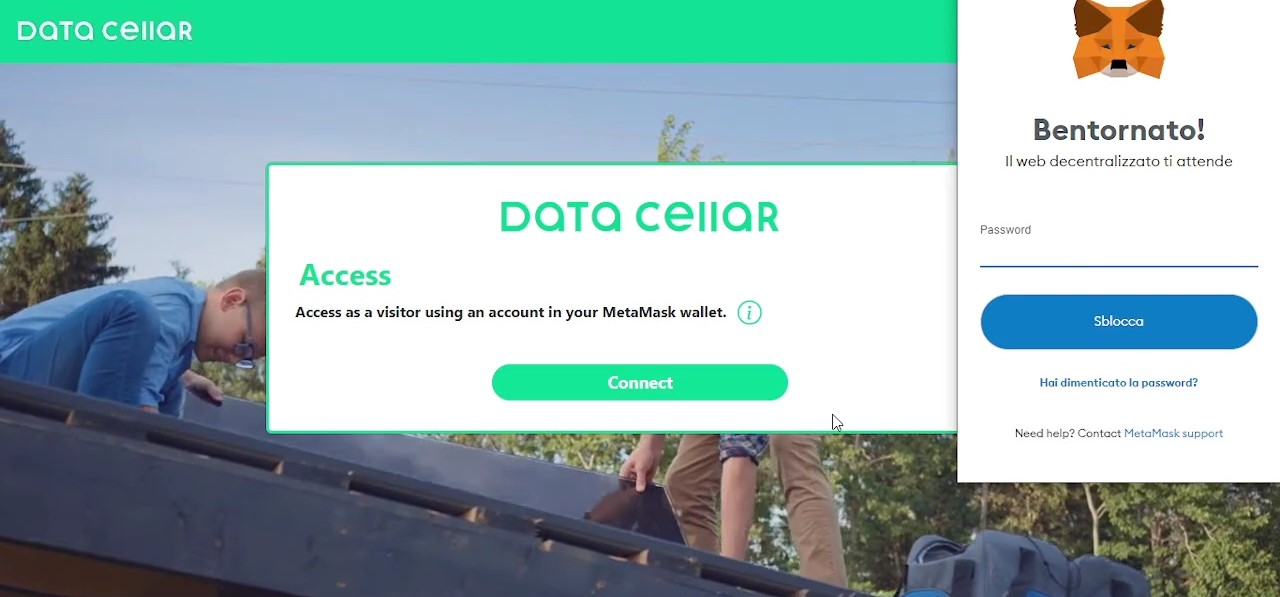
\includegraphics[width=1\textwidth]{Images/c6_1.jpg} 
  \caption{Process to create a cryptographic proof.}
\end{figure}

\subsection{Sign-Up Procedure}

This step in the process allows the user to register with the selected account within the MetaMask wallet and using one of the blockchains, in which the smart contract that 
serves as the registry for the \gls{dapp} has been previously deployed.

To begin, the user must fill in all the fields on the form presented to him; every value entered by the user is properly validated, so as to prevent possible security 
problems, but this still does not fully follow the \gls{ssi} paradigm. This is because there are currently no authentic \gls{vc}s from which to take this data (as 
explained in detail in the previous section). This data will constitute the \gls{vc} payload, which the \gls{dapp} browser, in the manner described above, will send through the 
server to the user.

Before receiving this \gls{vc}, however, the user must register by adding his account in the \gls{dapp}'s smart contract, which serves as a registry, present on the referenced 
blockchain. To do so, he must make a transaction, via the MetaMask wallet, which will involve payment of fees, both from MetaMask and from the network used. This 
registration is necessary not only to allow the application administrator to know how many users are registered and with which accounts, but also to control and issue only 
one \gls{vc} per account.

\lstinputlisting[language=JavaScript]{Codes/register.js}

Once the registration is completed, the \gls{vc} will be provided to the user who, at the push of a button, can download it to his device and store it securely, as indicated.

\begin{figure}[h]  
  \centering
  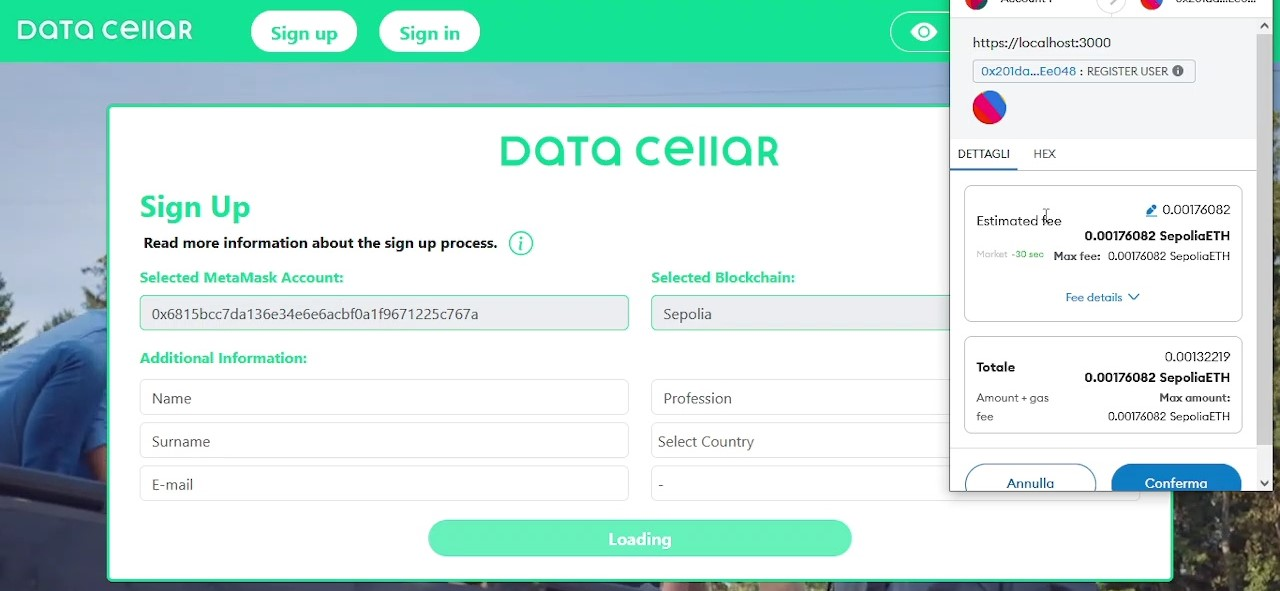
\includegraphics[width=1\textwidth]{Images/c6_2.jpg} 
  \caption{Process to create a cryptographic proof.}
\end{figure}


\subsection{Sign-In Mechanism}

In this final and perhaps most important step, user authentication occurs, using the account selected within the MetaMask wallet and the blockchain with which the 
registration was made. A note reminds the user to change the network selected in the MetaMask extension in case it is incorrect.

To do this, the user must provide the \gls{vc} issued during the sign up phase, from the browser \gls{dapp}, for the selected Ethereum account; this is because there is 
currently no way to request the corresponding \gls{vp} (as explained in detail in the previous section). The \gls{dapp} will then check the validity of this \gls{vc}, following the 
methods described above, to ensure both that it has been issued by the \gls{dapp} and that it contains the \gls{did}, associated with the account selected by the user, in his 
MetaMask wallet, at that time.

\lstinputlisting[language=JWT]{Codes/vc.jwt}

If these checks are passed, the user will be asked to sign a message containing a \gls{nonce}, using the private key associated with their account, through the MetaMask wallet. 
This process does not involve any transactions on the blockchain and therefore does not require payment of fees. As explained earlier, this \gls{nonce} serves to increase the 
level of security and will be automatically sent to the server along with the signed message and the payload extracted from the \gls{vc} previously provided by the user. After 
appropriate verification, if successful, the server will return a signed \gls{jwt} containing the payload received.

Finally, this \gls{jwt} will be placed in a token in the session cookies and the user will be authenticated. This corresponds to accessing the \gls{dapp} as a member. In this 
way, the user can view the entire browser \gls{dapp}, access its page, and perform all functionality, within the limits of the information in the session cookies. In fact, 
depending on the functionality the user wishes to perform within the \gls{dapp}, the session cookie token will be decoded and, based on the information obtained, certain 
authorizations will be granted or denied to the user. In addition, a button will appear in the navigation bar that allows the user to log out of the account with which they have authenticated.

\begin{figure}[h]  
  \centering
  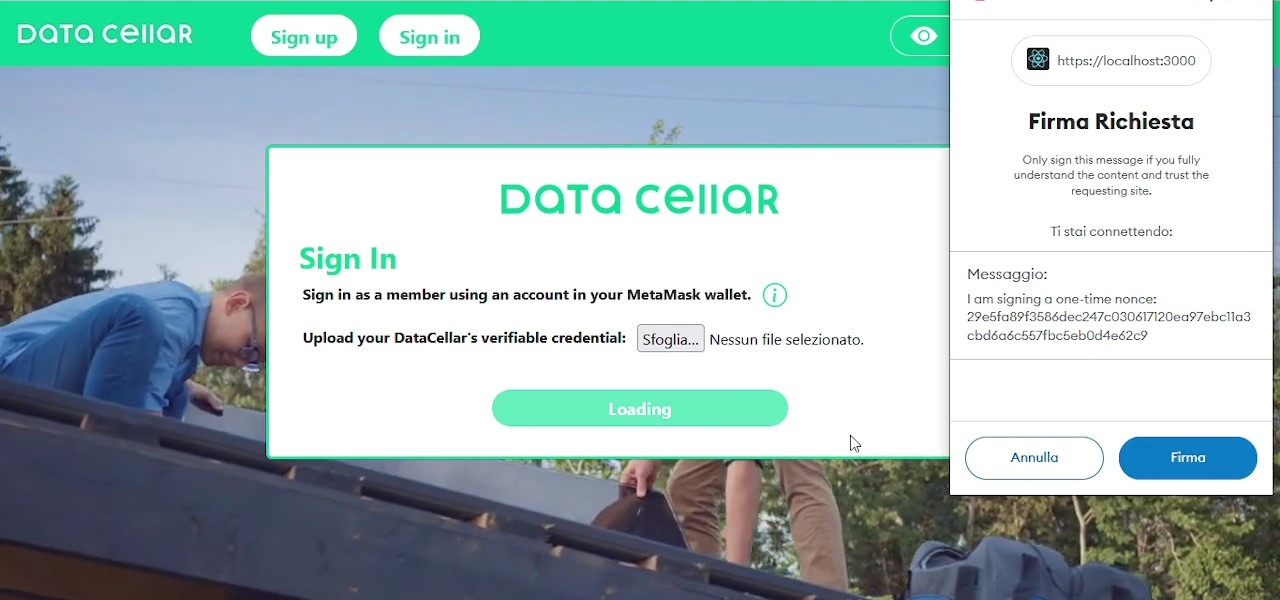
\includegraphics[width=1\textwidth]{Images/c6_3.jpg} 
  \caption{Process to create a cryptographic proof.}
\end{figure}

